\documentclass[a4paper,12pt,notitlepage]{article}
% \documentclass[letter,12pt,notitlepage]{article}% USA Letter

% Input
%\usepackage[latin1]{inputenc}
%\usepackage[T1]{fontenc}
\usepackage[american]{babel}

% References
\usepackage{url}
\usepackage{natbib} % Mandatory with acmtrans.bst
\usepackage[colorlinks,dvipdfm]{hyperref}
\hypersetup{
  linkcolor=blue,
  citecolor=blue,
  urlcolor=blue,
  pdfstartpage=1
}

% Graphics
\usepackage{graphicx}

% Math
\usepackage{amsmath}
\usepackage{bm}
\usepackage[binary]{SIunits}


\begin{document}

\title{Mesh Motion in NEMO}
\date{\today}

\maketitle

\begin{abstract}
  NEMO has the ability to calculate mesh motion in deforming domains,
  so that cell quality is maximized while the computational boundaries
  move. In order to maintain mesh quality, vertex motion is calculated
  using a multi--step strategy based on optimization of surface and
  volume meshes.  Because a single inverted cell can cause an
  expensive calculation to crash, this approach is designed to
  maximize the quality of the worst cell in the mesh.  The algorithm
  presented here is capable of handling significant
  motion without connectivity changes.  For the ability to handle unlimited motion, topological adaptation connectivity will be  required. The following text explains the design and strategy of the mesh motion code.
\end{abstract}

\medskip

\section{Introduction}
When CFD is required in a deforming domain, several mesh strategies
are available.  In static mesh approaches, the cells are truncated or
body forces are used to represent walls.  If, instead, the mesh moves
and deforms with the domain, then the CFD code can employ standard
control--volume techniques and requires only two extensions: (1) an
additional flux term to represent the motion of the faces relative to
the local velocity field and (2) the calculation of the change in cell
volume.  These relative fluxes must be calculated in a manner that is
consistent with the calculation of volume in order to exactly satisfy
Leibnitz's theorem (\cite{Quan:JCP2007}). The challenge then becomes how to move
vertices on surfaces and in the interior so that the mesh quality is
maintained at adequate levels.  The mesh moving algorithm must be
extremely robust, because a single bad cell is sufficient to halt the
CFD calculation.

The traditional way of calculating mesh motion is using Laplacian
smoothing. In this case, we set each point to a location that is the
average location of all the neighboring cells, as indicated in
Eqn. \ref{eq:LaplacianSmoothing}.

\begin{equation}
  \label{eq:LaplacianSmoothing}
  \overrightarrow{x} ={1 \over N_{neighbors}} \sum_{neighbors} \overrightarrow{x} _{i}
\end{equation}

On a regular mesh, Eqn. \ref{eq:LaplacianSmoothing} is exactly the
same finite difference equation that occurs if one solves Laplace's
equation for each of $x$, $y$, and $z$.  The resulting equations can
also be thought of as finding the equlibrium position of a network of
springs connecting each vertex along cell edges.  For a constant
spring stiffness and zero equilibrium length, the resulting equation
produces an unweighted averaging of vertex locations.

Laplacian smoothing is fast, simple, and easy to parallelize.
Unfortunately, it is not tied directly to any measure of mesh quality.
As a consequence, Laplacian smoothing frequently inverts cells,
especially in tetrahedral meshes.  In hexahedral meshes, even in unstructured cases, the conectivity is fairly regular.  The
number of cells sharing a vertex does not vary too far from the median
value of eight.  The angles between abutting cell edges, which act as
springs in Laplacian smoothing, vary from the ideal of
\unit{90}\degree, but not nearly to the degree found in tetrahedral
meshes.  In tetrahedral meshes, the number of cell edges ``pulling''
on a vertex varies very widely.  The directions of the edge
connections also vary, and will occasionally be, by chance, strongly
biased to one side of a vertex location.  As a consequence, Laplacian
smoothing normally tangles tetrahedral meshes.  The work of
\cite{lucchini:sae2007}, based on a finite--element smoothing
process, is one of the few known examples where a form of Lagrangian
smoothing has proven useful for calculations as complex as engines.  They have demonstrated parallelized moving mesh computations with unstructured hexahedral meshes.

Some attempts have been made to improve the performance of Laplacian
smoothing by using varying spring constants and non--zero equilibrium
spring lengths (\cite{Anderson:JCP2005}).  These methods can improve the performance
of Laplacian smoothing by making spring stiffness and equilibrium
length dependent on some indicator of mesh quality.  This approach is
not easy; if edges end up in compression instead of tension, the
system of equations may be unstable or result in twisted meshes.
Also, it is difficult to find a method for making spring stiffness
appropriately dependent on cell quality.

The approach used here is to view the process of mesh smoothing as an
optimization problem.  We wish to maximize the quality of the worst
cell in the mesh.  This methodology is consistent with the fact that
the success or failure of a calculation is largely
determined by the behavior of the worst cell.  In contrast, the C++
Mesquite\footnote{\url{http://www.cs.sandia.gov/optimization/knupp/Mesquite.html}}
library optimizes a smooth measure of global cell quality
(\cite{mesquite:freitag,mesquite:brewer}).  The trade--off is that the
global optimization of a smooth measure (such as an $L^{2}$ norm of
quality) is very fast, while point--wise optimization is more directly
tied to the quality of the worst cells.

Ideally, the location of all the mesh vertices would be optimized
simulataneously.  However, finding a truly global optimum is prohibitively expensive.
The point--wise approach is adopted here using the
OptMS\footnote{\url{http://www-unix.mcs.anl.gov/~freitag/Opt-MS/}}
library (\cite{optms:manual}).  Because the surface mesh serves as a
boundary condition for the interior mesh, the surface mesh is
optimized first.  Next, the interior mesh is optimized.

In point--wise optimization, the location of each mobile vertex is considered independently of the larger mesh.  The vertex location is chosen to optimize the quality of the local sub-mesh, that consists of cells that are directly connected to the mobile, or "free" vertex.  Thus, optimization is reduced to a local calculation.

A challenge for both interior and surface optimizaiton originates
from the goal of improving the quality of the worst cell.  For
both the interior and surface mesh smoothing, the quality function
does not have a continous first derivative, which also presents
difficulties.  The reason for this difficulty is that the optimization
problem is of the form shown in Eqn. \ref{eq:min_max}.

\begin{equation}
  \label{eq:min_max}
  f=max \left\lbrace min \left\lbrace q_i \left(
        x\right)\right\rbrace \right\rbrace
\end{equation}

Equation \ref{eq:min_max} indicates that we seek to optimize the
qualities in the local sub-mesh, numbered from $i=1 \mbox{ to } N_{cells}$, by varying the
free vertex location..  As
the vertices move, the identity of the worst cell will change
discontinuously.  An illustration of this shift is shown in
Fig. \ref{fig:min_max} for motion of a vertex, in the center of
Fig. \ref{fig:submesh}, in the $x$--direction.  The figure shows a
local sub--mesh of cells sharing a common vertex, which is illustrative
of how the actual optimization is done.  Since only the qualities of
abutting cells depend on the location of a vertex, the optimization is
done individually for each vertex, producing a local optimization.
The position of the
free vertex is chosen to maximize the minimum quality in the
sub--mesh.

\begin{figure}
  \centering
  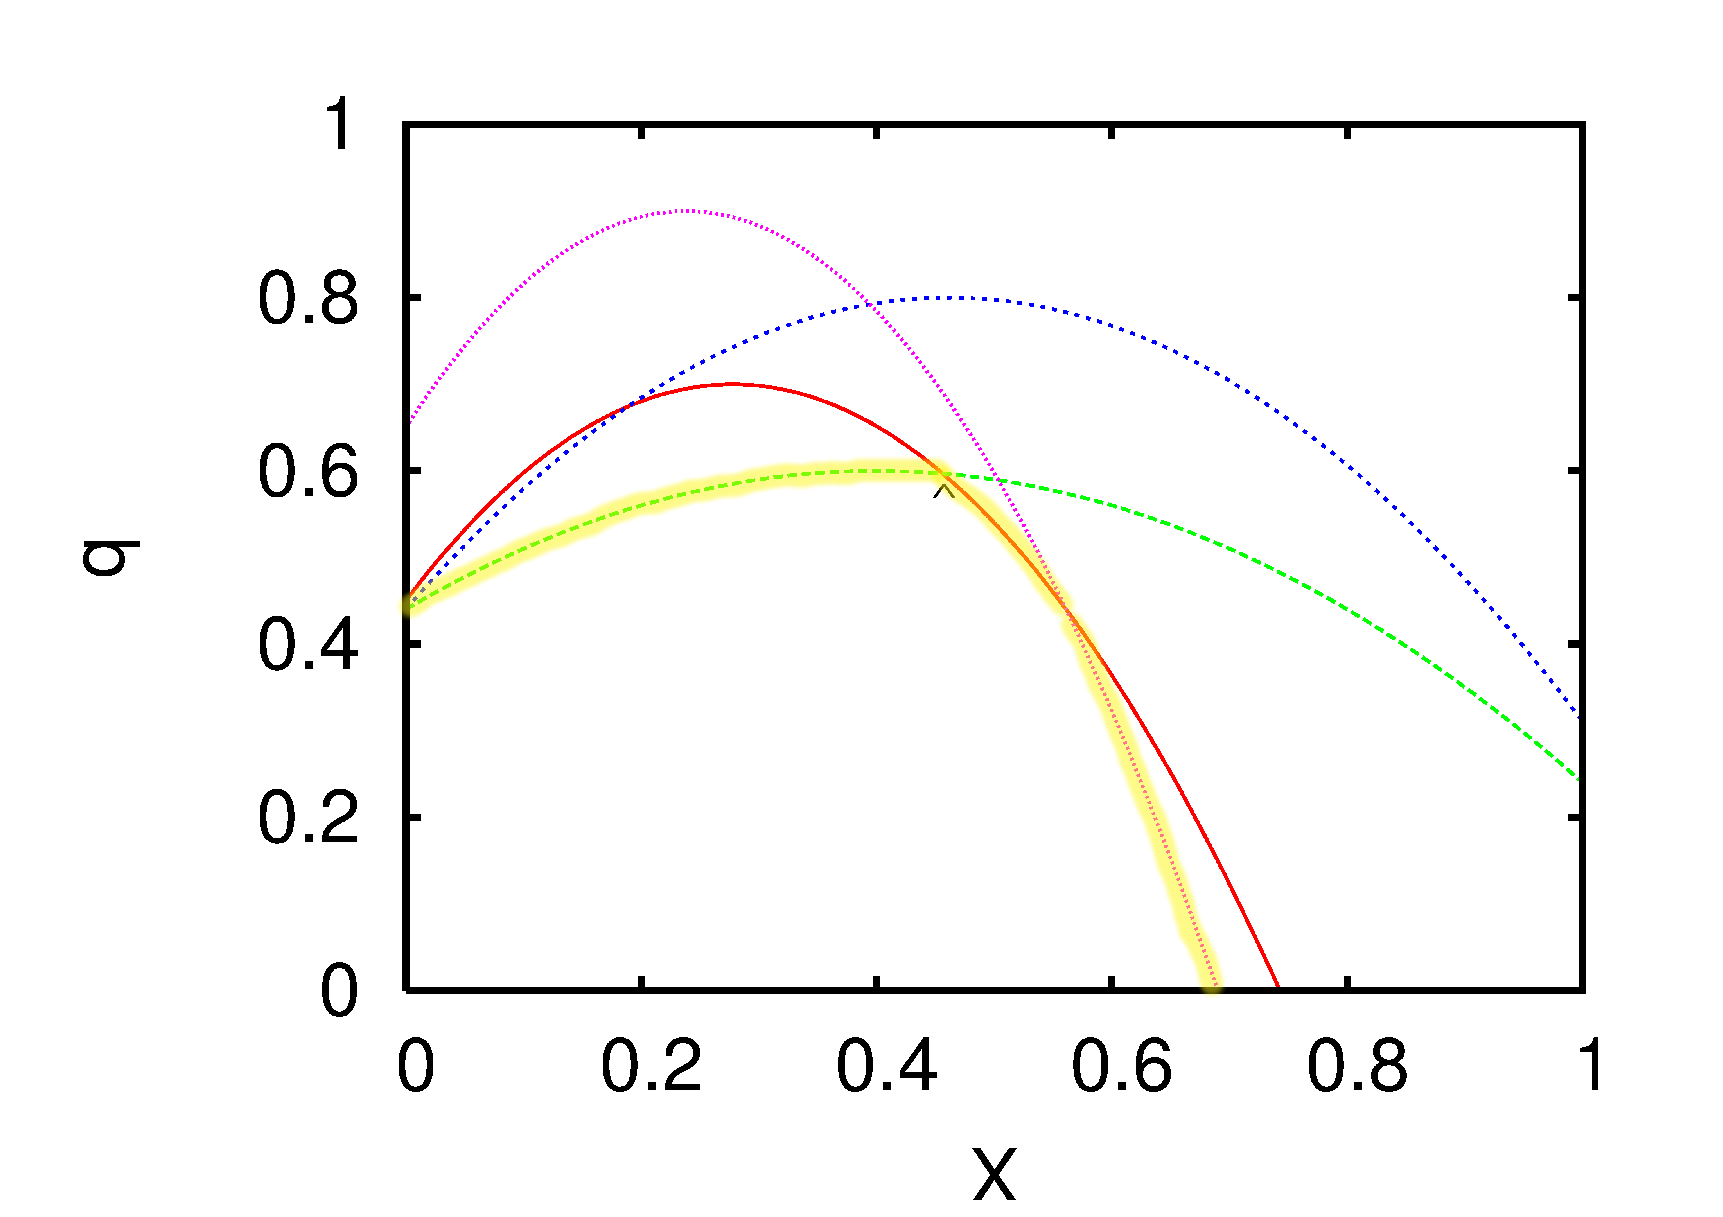
\includegraphics[width=0.9\textwidth]{Images/qplot.eps}
  \caption{The quality of several cells as the $x$ position of the free
    vertex is varied. The yellow highlighted composite curve shows the minimum of all the cell
    qualities as a function of $x$, and the carret  indicates the
    optimum.}
  \label{fig:min_max}
\end{figure}

\begin{figure}
  \centering
  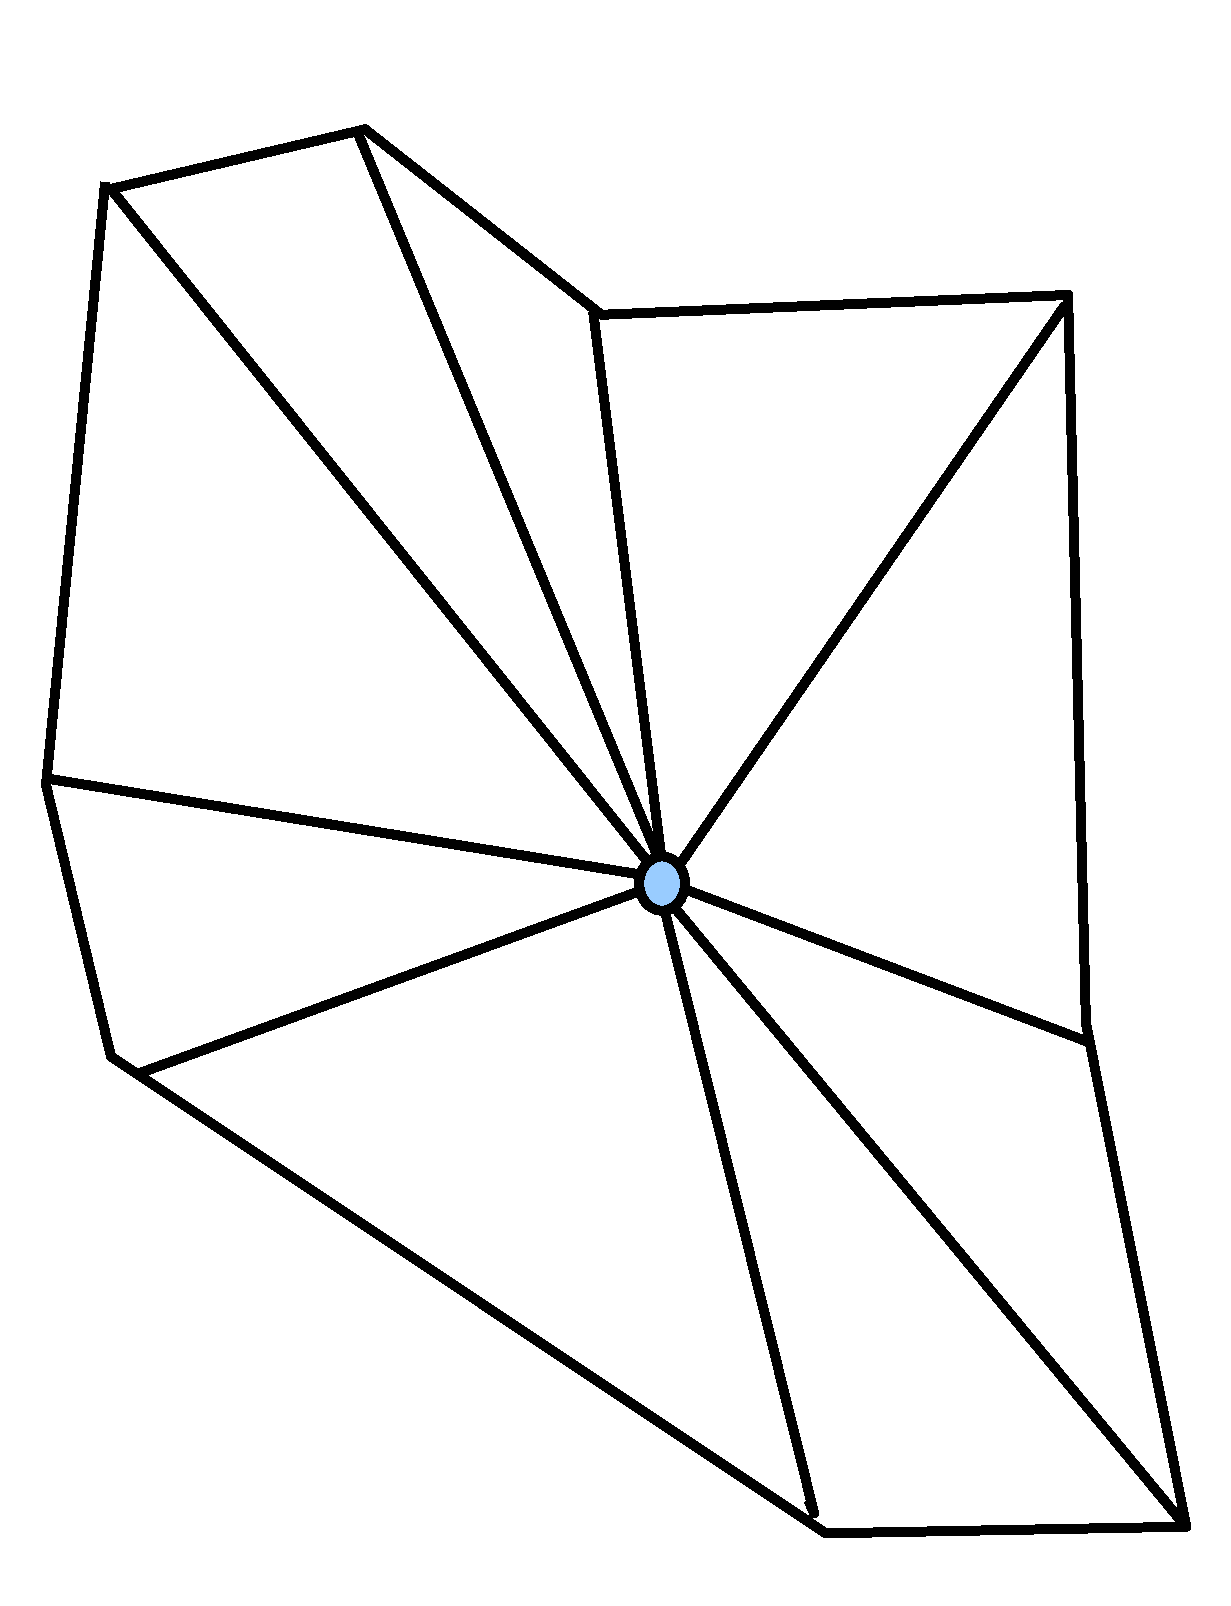
\includegraphics[width=.4\textwidth,height=.4\textwidth]{Images/submesh.eps}
  \caption{A local, two--dimensional, triangular sub--mesh.  The free
    vertex is marked with a circle.}
  \label{fig:submesh}
\end{figure}


\section{General Approach}
There are three phases to the mesh smoothing process.  They are (1)
Surface optimization--based smoothing, (2) Lagrangian smoothing of the
interior, and (3) Interior optimization--based smoothing.  The
inclusion of Lagrangian smoothing is not necessary, but can
accellerate the optimization process (\cite{optms:manual})

Because a good--quality surface mesh is necessary for maintaining the
quality of the interior mesh, our process begins by optimizing the
surface mesh.  Where possible, the surface mesh vertices are moved
along surfaces so that the surface mesh quality is optimized.  This
tangential movement of vertices is distict from the Lagrangian
movement of vertices on moving surfaces.

For any moving surface, Lagrangian motion of the vertices allows the
surface mesh to move rigidly with the surface. The quality of the
surface does not change, since, in the reference frame of the moving
surface, the vertex positions are not changing.  We refer to these
vertices as ``stick'' vertices, since they stick to the moving surface.

However, in many cases, one can optimize the surface mesh by allowing
vertices to slide along the surface tangent.  Not all surface vertices
are free to ``slide.''  In order to maintain the integrity of
the surface, a mathematical description of the surface is required.
This restriction is because curved surfaces must be projected onto
flat planes for two--dimensional optimization.  Once the new position
of the free vertex is calculated, the new vertex location must be
translated back into the corresponding location on the curved surface.

This optimization on surfaces can be considered a three-dimensional optimization that is constrained to  two-dimensional curved surfaces.
 The mesh points are constrained to
slide along surfaces, but unless the surface happens to be a plane,
the tangent of the surface will vary with the location of the vertex.
Thus surface mesh optimization is more complex than in the interior optimization, since the directions in which points can move is a function of where the points are currently located.

If significant discretization error occured during the calculation of
the new vertex position, then the location of the boundary vertices
could drift from the true surface over time.  If the surface is
recognized as a plane or cylinder, the vertex location can be can be reconciled with the
canonical surface (\cite{mesquite:freitag}).  So unless a precise mathematical
description of the surface is available, then the surface points are
constrained to stick to the surface.  If the surface can be described
as a cylinder or plane, then the points can slide relative to the
surface and yet remain precisely on the surface.  An example of
optimizing ``sliding'' vertices is shown in
Fig. \ref{fig:curved_surface}.

\begin{figure}
  \centering
  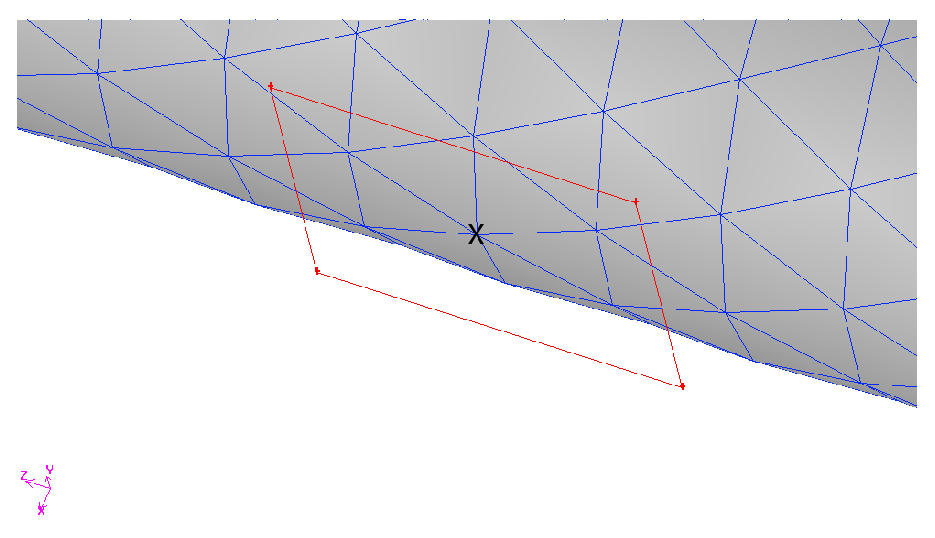
\includegraphics[height=.4\textwidth]{Images/curved_surface.eps}
  \caption{The mesh points, on a cylinder surface, are projected to
    the local tangent plane.  The plane is defined by the tangent at the location of the free vertex, denoted by the X.}
  \label{fig:curved_surface}
\end{figure}

In the example shown in Fig. \ref{fig:curved_surface}, the free vertex and surrounding vertices will be projected to the tangent plane.  The free vertex's location will be optimized, which moves it slightly off the cylindrical surface.  The vertex will then be moved in the direction normal to the cylinder, placing it back on the cylinder surface.  This process lets vertices slide without degrading the representation of the surface.

In order to reduce the required effort and likelihood of mistakes in
performing moving mesh calculations, we have implemented a very
convenient ``automatic surface recognition'' algorithm.  This
algorithm, with no user inputs other than the mesh, recognizes
canonical surface shapes, such as a plane or cylindrical surface. The
surface need only conform to any portion of an infinite plane or
cylinder (e.g. the algorithm recognizes a curved surface that might be
only twenty degrees of a cylindral surface).  The algorithm uses a
least--squares fitting process to test every surface.

For a plane, the least-squares fit requires the solution of a linear system of four equations.  The procedure for fitting more general surfaces requires an iterative approach.  In the code, treatment of a more general surface is demonstrated by recognizing cylindrical surfaces.  A general cylinder equation is represented by an infinite cylindrical surface with rotation and translation.  The Levenberg-Marquardt algorithm is used to find the cylinder orientation, location, and radius that best fits the surface points (\cite{SLATEC:Vandervender}).  This fitting is performed only once; if a surface moves during the calculation, the constants representing the cylinder or plane position are updated analytically.

Currently, only
recognition of planes and cylinders have been implemented, however
extensions for spheres or cone frustra are possible.  If the surface
is neither a plane or a cylinder, then the algorithm tags the surface
as ``unrecognized'' and moves on.  An example is shown in Fig. \ref{fig:Surfaces}.  Only recognized surfaces may have
sliding vertex optimization, since the surface normal of an
unrecognized surface cannot be known exactly.

\begin{figure}
	\centering
	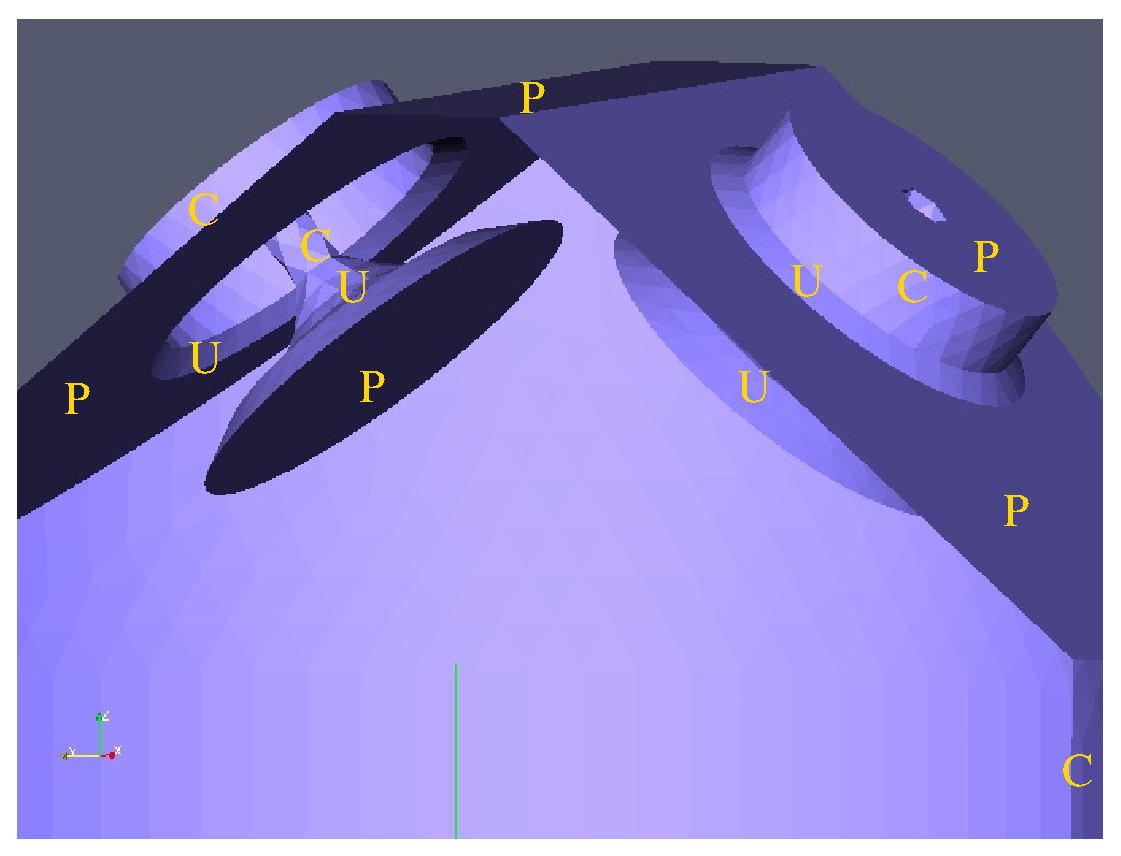
\includegraphics[height=0.4\textwidth]{Images/surfaces.eps}
	\caption{A cut-away view of a cylinder and four-valve engine showing automatically recognized surfaces..  Cylindrical surfaces are denoted with "C", planar with "P", and unrecognized with "U."}
	\label{fig:Surfaces}
\end{figure}

After the optimization of the surface mesh, the interior mesh is
optimized.  This can be done with direct application of analogous
methods to those used in the two--dimesional phase.  However, it may be
expedient to use Lagrangian smoothing to provide a provisional mesh
solution.  The results of the Lagrangian simulation are adequate for
the great majority of the cells.  A small percentage of the cells will
be tangled or very low quality.  The optimization phase of the
interior phase follows.  The interior mesh is untangled as it is
optimized using several iterative sweeps through the interior.  The
final result will be a high--quality mesh, so long as the limitations
of the algorithm are respected.

The ability to untangle meshes is fairly uncommon and is quite
helpful.  Tangled meshes have negative volumes and present difficult
mathematical problems for optimization algorithms.  The current
approach for untangling is based on a linear programming method to
find a location of the free vertex where all cell volumes are positive
(\cite{optms:manual}).  If the local sub--mesh is sufficiently tangled, a
solution may not exist and the untangling method will fail.  However,
by using repeated sweeps through the domain, a region of tangled cells
will gradually be untangled, as the untangling algorithm finds valid
vertex locations for the less tangled cells.

The untangling capabilities of the code are quite important.  This
means that invalid initial meshes can be repaired and, if inverted
cells occur as a result of the Lagrangian vertex solution, they can be
repaired.  The outcome of the untangling process is usually a
low--quality sub--mesh, but using several optimization passes will
usually bring the mesh up to an acceptable quality.

\section{Code Structure}
The NEMO code, in which we have demonstrated the moving mesh
capapability, is an inherently parallel software library built using
object--oriented Fortran 95 (\cite{toninel:phd}).  NEMO is designed as
a set of foundation classes upon which specific applications can be
built, similar to the approach of
OpenFOAM\footnote{\url{http://www.opencfd.co.uk/openfoam/}}
(\cite{weller:foam}).  Much of the lower level mesh smoothing for
surfaces and interior points is based on a modified version of the OptMS library developed
by Freitag (\cite{optms:manual}).  The resulting code is fully parallelized,
after an initial domain decomposition, using an ``owner computes''
paradigm.

Initially, the mesh is read in by all processors, and any recognizable
surfaces are noted.  Data structures, unique to the PSBLAS library,
are initialized at this point.  These data structures facilitate
parallel communication about mesh entities and allow solutions of
equations at cell centers, verticies, or face centers.  Decomposition
is handled by the ParMetis\footnote{
  \url{http://www-unix.mcs.anl.gov/~freitag/Opt-MS/}} library
(\cite{parmetis}), after which, each processor only holds the local
mesh in memory, with halo layers of cells, faces, and vertices.  This
halo layer, which can be of arbitray depth, provides a copy of the
recent state of the mesh that lies on neighboring processors and abuts
the processor boundary.  The halo management is based on the
PSBLAS\footnote{\url{http://www.ce.uniroma2.it/psblas/}} library
(\cite{filippone:psblas,buttari:phd}), which can keep data
synchronized and exchange information with a higher--level interface
than MPI provides.

As time advances, first the surfaces are moved with the associated
surface mesh.  Next, the sliding surface meshes are optimized using
the two--dimensional capabilities of the OptMS library.  Repeated
sweeps are made over the surface as the optimization is done
point--wise.  Laplacian smoothing then provides an initial guess of the interior vertex positions.  Several optimization passes then completes the mesh optimization.  The steps, as described in detail below, are listed here:

\begin{enumerate}
\item Move surfaces and associated points
\item Untangle and optimize surface meshes
\item Lagriangian interior smoothing
\item Interior untangling and optimization
\end{enumerate}

Each of these steps is described in detail below.

\subsection{Moving Surfaces and Associated Points}
When a surface, such as piston face or valve, moves, the points that lie on that surface should move as well.  In general, the points are moved in a Lagrangian fashion.  If a surface is of a recognizable type, such as a plane or cylinder, the mathematical representation of the plane and cylinder are moved as well.

\subsection{Untangle and Optimize Surface Meshes}
The sliding mesh optimization first projects the vertices to a tangent
plane.  Unlike a typical trigonometric projection, a length--preserving
projection is used, as shown in Fig. \ref{fig:projection}.  The
length--preserving projection better represents the edges in the plane.
The $x$ and $y$ positions of each vertex in the local surface sub--mesh are
calculated in a local two--dimensional coordinate system that has the
origin located at the free vertex.

\begin{figure}
  \centering
  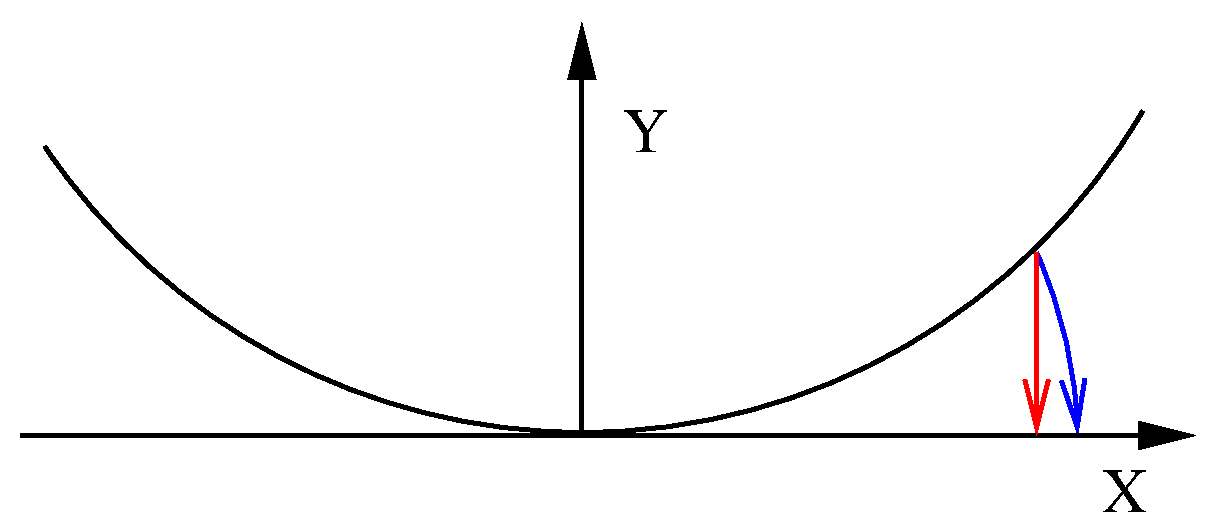
\includegraphics[width=0.9\textwidth]{Images/projection.eps}
  % figProjection.eps: 300dpi, width=4.82cm, height=2.02cm, bb=0 0 569
  % 238
  \caption{The projection of a point to a tangent plane, as seen from
    the side.  The red line shows the trigonometric projection and the
    blue arc shows the length preserving projection.}
  \label{fig:projection}
\end{figure}

Because the OptMS library only supports optimization of simplices
(triangles and tetrahedra), the algorithm checks first to see if the
free vertex is shared only by triangles.  For any other kinds of
cells, the vertex location, in the tangential plane, is set to the
average location of the neighboring vertices.  Because optimization
must be preceeded by untangling if any cells in the sub--mesh are
inverted, the algorithm also checks that all the cells in the surface
sub--mesh are valid.  If any local cells are tangled, then untangling
is applied, otherwise the optimization routine is called.  The OptMS
library applies optimization to the vertex using a scheme analogous to
steepest descents, but generalized for the non--smooth problem
represented in Fig. \ref{fig:min_max}.

\subsection{Lagrangian Interior Smoothing}
Once the surface mesh is smoothed, the interior vertex positions are
calculated using Laplacican smoothing.  This calculation is performed
separately for the $x$, $y$, and $z$ coordinates, which are each
independent equations.  The matrix is exactly the same for all three
equations, so the matrix and pre--conditioner data are re--used.  The
parallel conjugate gradient solver in PSBLAS, with ILU
preconditioning, typically converges in about five to ten iterations.
The resulting mesh often contains a small number of unacceptable
cells, but the computational cost is very low, and it provides a good
estimate of the final mesh.  Unlike the local point--wise optimization,
the Lagrangian smoothing communicates information globally.

The boundary conditions used in the Laplacian smoothing are all
Dirichlet.  It is assumed that all surface points will remiain where
the surface smoothing put them.  If the interior mesh vertices lie at
a boundary between two different kinds of cells, such as tetrahedra
and hexahedra, then the vertices are also fixed during this stage.
The reason for fixing these interior vertices is that Lagrangian
smoothing is overly biased by the number and orientation of edges.
At the transition between hexahedral and tetrahedral cells, the
greater number of edges present in the tetrahedral region will pull
the vertices towards the tetrahedral region, which may not be
desirable.  As a consequence, the boundaries between two kinds of
cells are not permitted to move in the current implementation.

\subsection{Interior untangling and optimization}
The final phase of optimization is the point--wise sweeps over the mesh
interior.   Depending on the kind of cells and the validity of the local sub-mesh, several different treatments of the vertex are applied. Consistent with the Laplacian smoothing phase, when vertices are connected to a mixture of cell types, the vertex is
left in place.  For vertices used by non-tetrahedral cells, simple averaging of locations is performed, equivalent to Laplacian smoothing.

For vertices that are used only by tetrahedra, true optimization is applied.  Because optimization must be preceeded by untangling when any
cells in the sub--mesh are inverted, the algorithm first checks that all
the cells in the sub--mesh are valid.  If any local cells are tangled,
then untangling is applied.   For valid local sub-meshes, containing only tetrahedra,
three--dimensional optimization using the OptMS library is
performed.  Between four to ten sweeps through the mesh interior are sufficent to achieve an optimally smoothed mesh.

\bibliographystyle{Bib/acmtrans}
%\bibliographystyle{Bib/asmems4}
%\bibliographystyle{plain}
\bibliography{Bib/nemo_doc}
\addcontentsline{toc}{section}{References}

\end{document}


@
